Las razones por las cuales se toma la decisión de fabricar la estructura del brazo 
mediante impresión 3D son:

\begin{itemize}
  \item Cumplir con el objetivo de replicabilidad y asequibilidad: una de las bases 
  del proyecto es que pueda ser reproducible a bajo coste tanto de recursos como 
  de tiempo. Se decide por tanto construir la estructura física del brazo mediante 
  técnicas de impresión 3D, ya que están altamente extendidas y son cada vez más
  asequibles.
  
  \item Características físicas del material: los plásticos utilizado en impresión 3D
  suelen ser ligeros y suficientemente resistentes para soportar las cargas para las 
  que está pensado el manipulador.
  
  \item Disponibilidad de impresora 3D: dado que la Universidad es capaz de proveer 
  al equipo con una impresora 3D, los costes del proyecto se abaratan si la estructura
  es realizada con los medios de los que la ya se disponen.
  
  \item Simplificar el proceso de mejora y personalización: debido a la naturaleza
  \ac{OS} y \ac{OH} del proyecto, se espera que las personas interesadas puedan 
  contribuir a él, mejorándolo y/o personalizándolo. Además, la impresión 3D facilita
  estas acciones.
\end{itemize}

En particular, la impresora que la Universidad pone a disposición del equipo de 
trabajo es la ``\textit{Ultimaker 3 Extended}'', la cual es capaz de imprimir en una 
alta variedad de materiales, de los cuales destacan los siguientes:

\begin{itemize}
    \item \ac{PLA} \cite{AcidoPolilactico2020}: este material permite imprimir 
    con alta precisión dimensional y una resistencia a la tracción excepcional, 
    el cual soporta grandes velocidades de impresión y es biodegradable, ya que
    se obtienen a partir de almidón de maíz, de yuca, mandioca o de caña de azúcar. 
    \item \ac{ABS} \cite{AcrilonitriloButadienoEstireno2020}: material que presenta 
    buena adhesión entre capas y una resistencia a temperaturas de hasta 
    $\numprint[\tccelsius]{85}$. Permite obtener buenos detalles estéticos.
    \item Ultimaker Nylon: este material es un tipo de poliamida basada en los 
    polímeros plásticos PA6/66. Presenta una absorción de humedad reducida así como 
    una capacidad considerable de resistencia ante tensiones mecánicas junto con un 
    bajo coeficiente de fricción, haciéndolo un material ideal para construcciones 
    mecánicas.
    \item CPE y CPE+: este material presenta una alta estabilidad dimensional, con 
    buena resistencia al impacto y a la temperatura. Debido a su alta solidez y su 
    estabilidad dimensional ofrece un buen rendimiento mecánico y gran resistencia 
    al desgaste.
\end{itemize}

Debido a la naturaleza mecánica del proyecto, el equipo ha decidido emplear 
materiales con alta resistencia mecánica para las piezas móviles. 
El Ultimaker Nylon junto con el CPE cumplen con dicha característica.

Por otro lado, los componentes que no sean móviles como carcasas o  
piezas protectoras se imprimirán en PLA ya que, tras realizar pruebas, el equipo 
de desarrollo ha concluido que el material es lo suficientemente resistente para 
soportar los pesos a los que será sometido.

\section{El proceso de impresión 3D}
El proceso de impresión 3D se compone de varias etapas y de bastantes pruebas hasta
que se consiguen resultados aceptables. En el momento de impresión, el brazo se
compone de unas 27 piezas, pero se han tenido que imprimir un total de 75 piezas,
lo que supone un $277.\overline{7}\%$ más en comparación con las piezas que componen
al \pArm{} (figura \ref{fig:tcb}).

\begin{figure}[H]
    \centering
    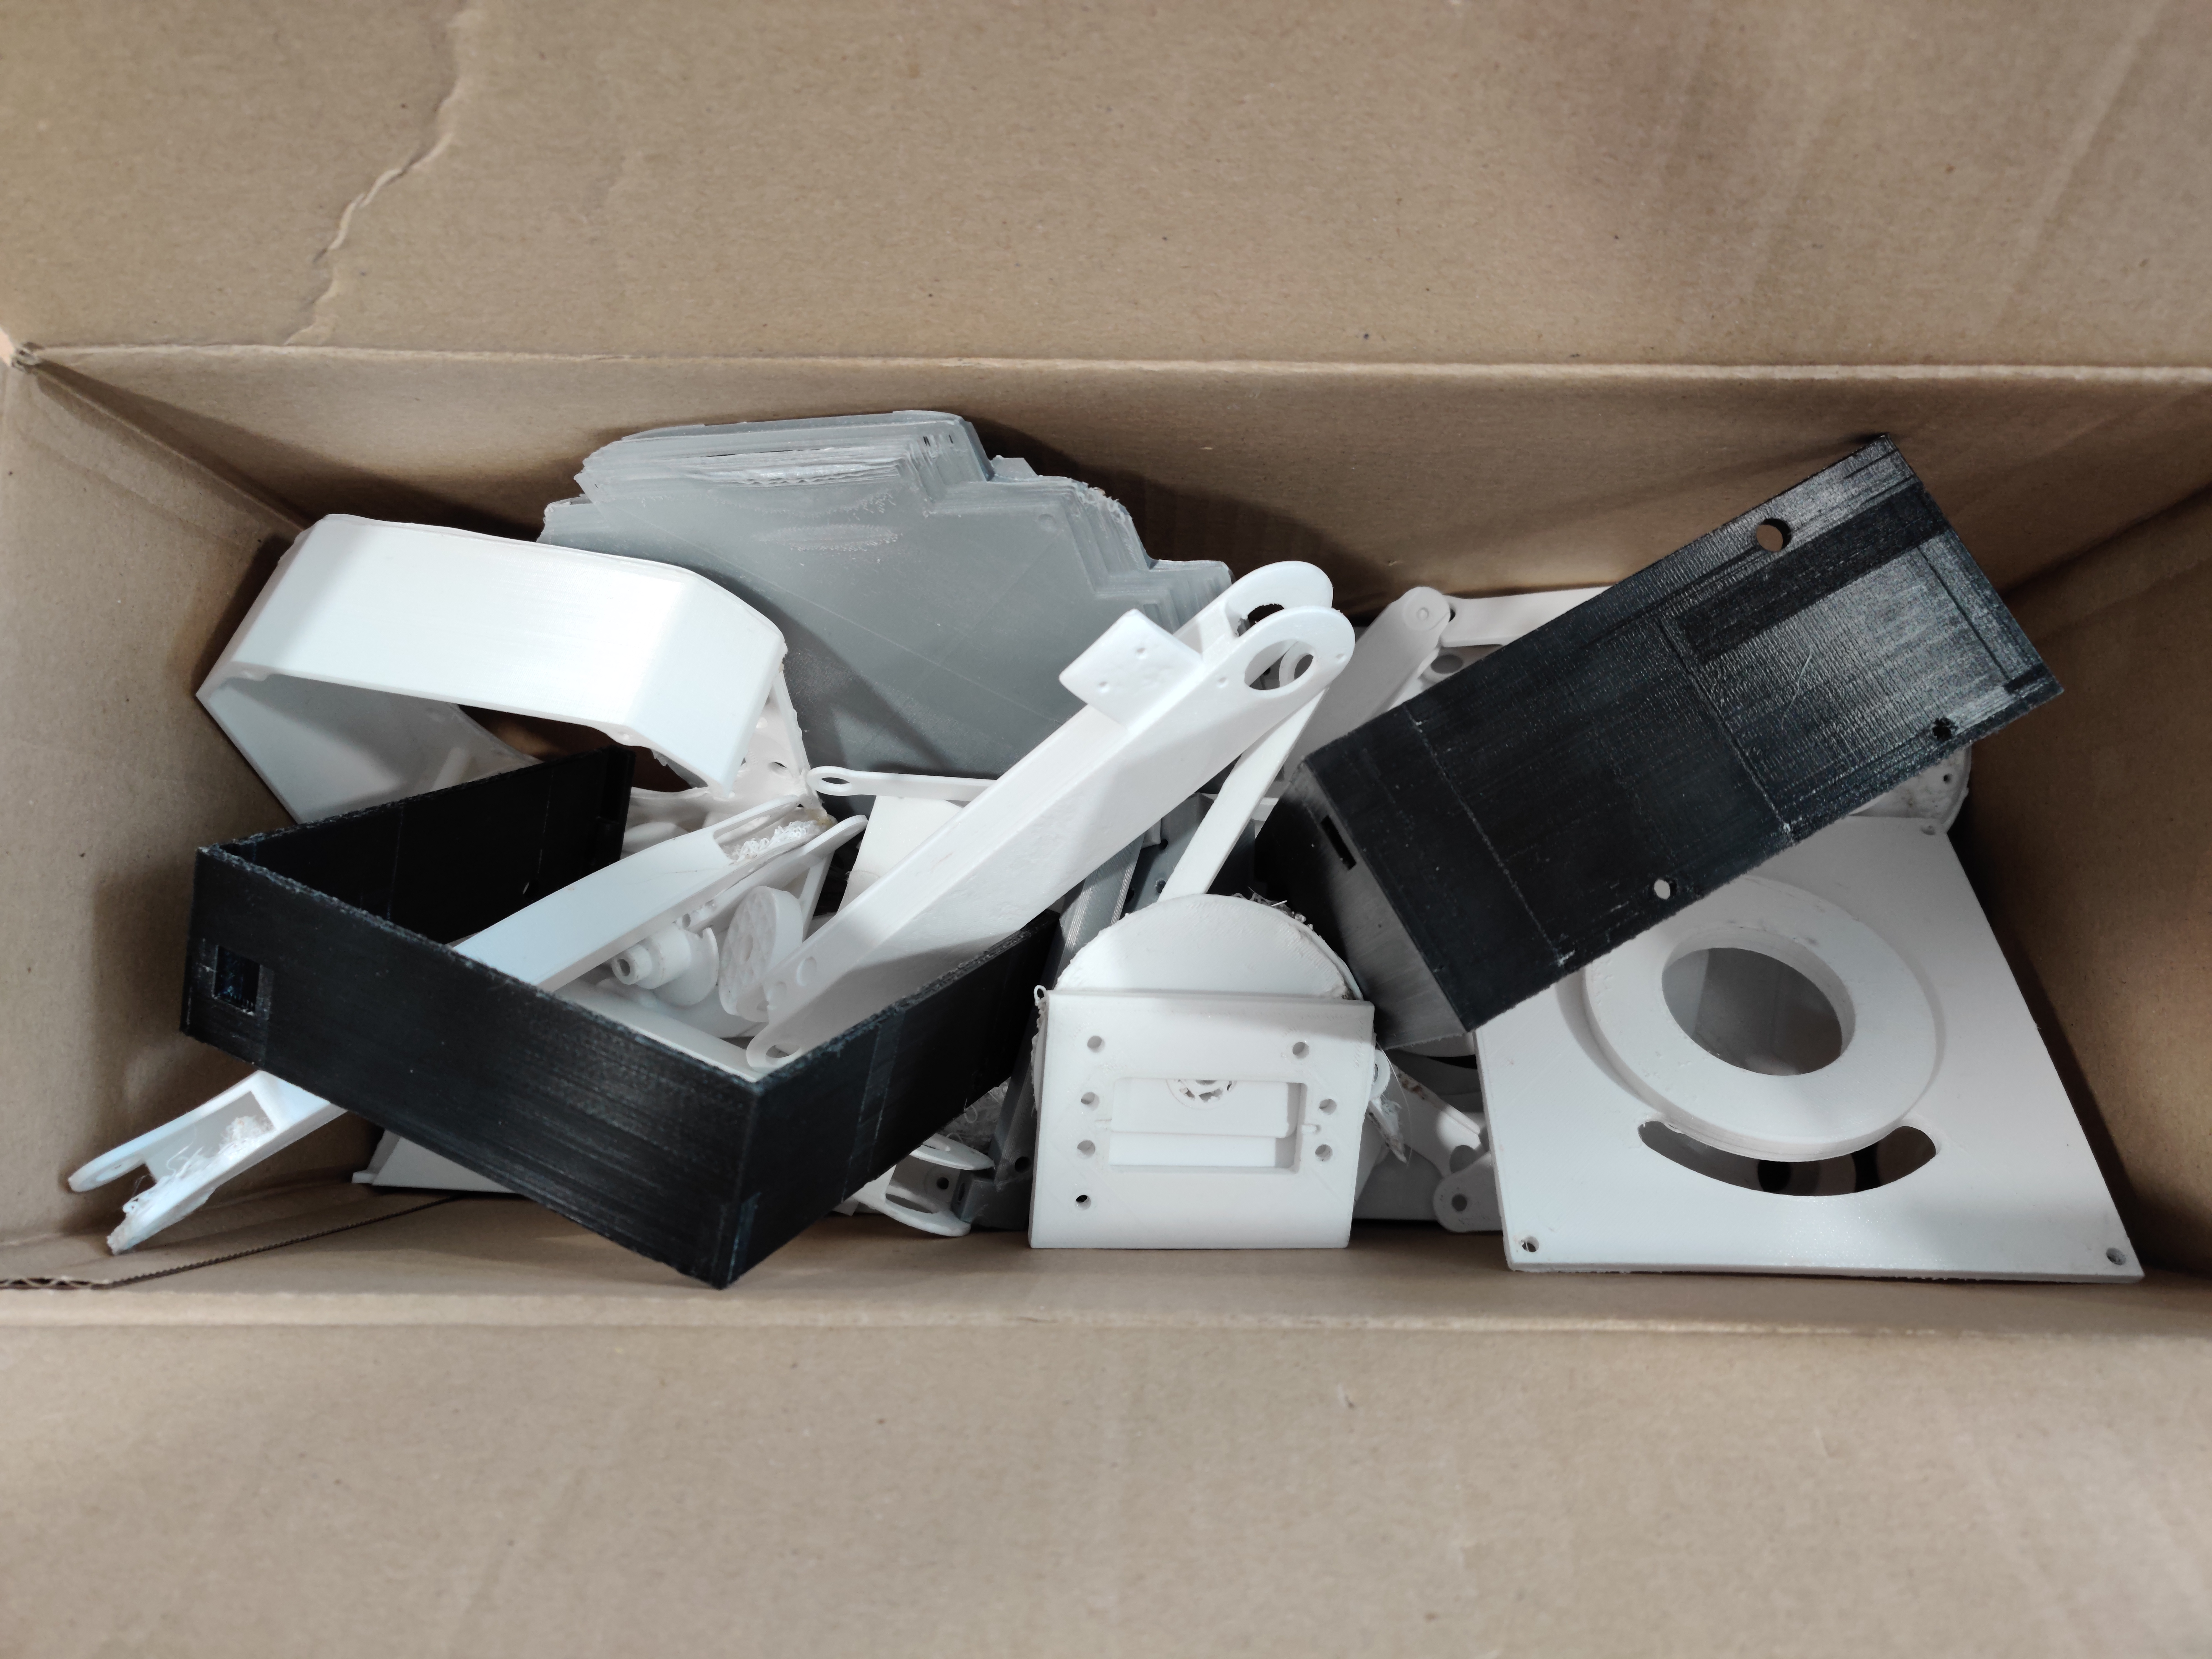
\includegraphics[width=.9\linewidth]{pictures/tcb.jpg}
    \caption{Algunas de las piezas que no se correctamente.}
    \label{fig:tcb}
\end{figure}

Dicha cantidad de piezas fallidas se ha producido por distintas causas:

\begin{itemize}
    \item Inexperiencia por parte del equipo de desarrollo, ya que era la primera vez
    que se trabajaba con impresoras de este estilo.

    \item Invalidez de las piezas originales: como se ha comentado en el apartado de
    diseño 3D (sección \ref{sec:3desing}), muchas de las piezas originales no eran
    válidas para ser impresas en 3D, por lo que fue necesario volver a imprimirlas
    tras comprobar que en efecto presentaban errores.

    \item Mal estado de uno de los \textit{nozzle} de la impresora, en particular,
    el cabezal tipo BB de $\numprint[mm]{0.4}$.

    \item Mal estado del material de soporte de \ac{PVA}, por lo que ciertas piezas
    no pudieron ser impresas.

    \item Falta de material de impresión para ciertas partes, como \ac{PVA} y \ac{CPE}.
\end{itemize}

Todos los sucedidos contratiempos se explican con mayor detalle en el apartado
\ref{sec:3derr}.

Tras las pruebas fallidas se fue perfeccionando el proceso de impresión 3D hasta llegar
al punto en que todas las piezas que se imprimían salían bien en el primer intento, lo
cual se explica a continuación.

\subsection{El entorno de impresión 3D}
El entorno de producción y preparación 3D es el Ultimaker Cura

\begin{figure*}[H]
    \centering
    \includegraphics[width=.5\linewidth]{pictures/Ultimaker_cura.png}
    \caption*{Logotipo de Ultimaker Cura \cite{CuraSoftware2019}.}
\end{figure*}

el cual ofrece una interfaz para poder posicionar piezas y realizar ajustes sobre
las mismas (figura \ref{fig:cura_gui}).

\begin{figure}[H]
    \centering
    \includegraphics[width=.9\linewidth]{pictures/cura_ui.png}
    \caption{Entorno de producción de Cura.}
    \label{fig:cura_gui}
\end{figure}

La herramienta se encuentra disponible para todas las plataformas y su descarga
puede hacerse desde la web oficial de Ultimaker\footnote{\url{https://ultimaker.com/es/software/ultimaker-cura}}.

Cuando se coloca una pieza, se ha de mover y preparar para ser impresa. La impresión
siempre se hace desde las capas inferiores hasta las capas superiores, por lo que es
posible imprimir múltiples piezas simultáneamente. Es recomendable que las piezas que
se impriman no asciendan muy rápido verticalmente, ya que eso implicará que se necesita
mayor soporte y estabilidad vertical. Por ejemplo, en la figura \ref{fig:vpiece_1} se
muestra una pieza que es casi completamente vertical, lo cual le supondrá un gran
esfuerzo a la impresora a la hora de mantenerla estable y asegurar que salga bien.

\begin{figure}[H]
    \centering
    \includegraphics[width=.7\linewidth]{pictures/vertical_piece1.png}
    \caption{Pieza del \pArm{} casi completamente vertical.}
    \label{fig:vpiece_1}
\end{figure}

Para poder imprimir la pieza en esa posición correctamente es necesario añadir material
de soporte ya que, en otro caso, es muy probable que se caiga.

Por lo general, es recomendable evitar el uso de dicho material por múltiples motivos:

\begin{itemize}
    \item Es un material especialmente caro: una bovina de $\numprint[g]{750}$ cuesta
    85.14\EUR{}, por lo que interesa no gastarlo rápidamente.

    \item Es un material muy sensible al ambiente: al ser disoluble, absorbe mucha
    humedad del ambiente y se acaba pudriendo si además está expuesto a la luz.

    \item A raíz de lo anterior, aunque el material parezca estar en buen estado, a
    la hora de imprimir pueden salir grumos de color oscuro, signos de que el material
    se ha podrido al ser expuesto a la temperatura del \textit{nozzle}.

    \item Del mismo modo, en una impresión de larga duración el \ac{PVA} se puede
    deteriorar con el tiempo, ya que estará expuesta a la temperatura constante del
    \textit{build plate} así como al flujo constante de aire de los ventiladores del
    cabezal de impresión.

    \item Al utilizar doble extrusor pero no funcionar a la vez, los tiempos de 
    impresión se multiplican ya que hay que recorrer dos veces la superficie que se
    ha impreso además de tener que dedicar tiempo a intercambiar los extrusores.
\end{itemize}

En el apartado \ref{sec:3derr} se explica con más detalle los problemas que se
encontraron al imprimir en 3D utilizando dicho material y las soluciones que se
plantearon.

Antes de utilizar doble extrusión para imprimir se puede modificar la posición
y orientación de la pieza desde el \ac{SW} de Cura para ver si se puede posicionar
de forma que pueda ser impresa con un único material. La pieza anterior puede ser
tumbada para que el crecimiento sea más progresivo, quedando de la siguiente forma
(figura \ref{fig:vpiece_2}):

\begin{figure}[H]
    \centering
    \includegraphics[width=.7\linewidth]{pictures/v_piece_2.png}
    \caption{Pieza del \pArm{} en otra posición para que sea más sencilla de imprimir.}
    \label{fig:vpiece_2}
\end{figure}

Pese a haber colocado la pieza en dicha posición, el \ac{SW} Cura indica que la impresora
puede tener problemas al crearla. Esto se muestra marcando el segmento que se considera
problemático de color rojo (figura \ref{fig:vpiece_err}):

\begin{figure}[H]
    \centering
    \includegraphics[width=.7\linewidth]{pictures/v_piece_err.png}
    \caption{El ``techo'' de la pieza se marca de color rojo.}
    \label{fig:vpiece_err}
\end{figure}

Esto es porque, al ser el ``techo'' de la pieza y al estar hueca, no hay una capa sobre
la que apoyar el material plástico que completaría la figura. Por ende, es necesario
añadir material de soporte (en \ac{PVA} o \ac{PLA}) de forma que se puede imprimir
correctamente la pieza (figura \ref{fig:vpiece_ok}):

\begin{figure}[H]
    \centering
    \includegraphics[width=.7\linewidth]{pictures/v_piece_ok.png}
    \caption{Con el material de soporte la pieza es imprimible.}
    \label{fig:vpiece_ok}
\end{figure}

Según el material en uso, se han de adaptar ciertas configuraciones para intentar que
las impresiones salgan bien, las cuales se detallan a continuación.

\subsection{Los parámetros de configuración}
Como se ha mencionado anteriormente, el \pArm{} está compuesto principalmente por:
\begin{itemize}
    \item \ac{PLA} para piezas de soporte, que no van a moverse sobre otras piezas.
    \item \ac{CPE} para piezas mecánicas que necesitan transmitir fuerzas a través
    de la estructura mecánica del brazo.
\end{itemize}

Para el primero de los materiales, la configuración básica que ofrece el \ac{SW}
Cura es suficiente, ya que es de los materiales más utilizados a la hora de imprimir.
En cambio, con el \ac{CPE} en conjunto con \ac{PVA} como material de soporte las
opciones de impresión han de ser configuradas con cierto rigor.

El material de soporte puede resultar bastante problemático en impresiones de larga
duración y acarrea consigo un mantenimiento que hay que realizar después de cada
impresión. Las impresoras Ultimaker necesitan tener conectados ambos extrusores
al cabezal de impresión, ya que utilizan el calor que pueden generar individualmente
para crear retroalimentación positiva entre ellos, esto es, se contribuyen mútuamente
para alcanzar la temperatura deseada (referencia en la imagen \ref{fig:um3_extruders}).

\begin{figure}[H]
    \centering
    \includegraphics[width=.5\linewidth]{pictures/um3_extruders.png}
    \caption{Vista del cabezal de impresión junto con los extrusores de la Ultimaker 3 \cite{Ultimaker}.}
    \label{fig:um3_extruders}
\end{figure}

Uno de los problemas de que el extrusor esté siempre contribuyendo a la temperatura
y al flujo de aire se produce cuando además tiene plástico \ac{PVA} en su interior.
Como se ha mencionado anteriormente, el \ac{PVA} absorbe con mucha facilidad la humedad
del aire y, al someterlo a calor, se pudre. Por ello, las impresiones de larga duración
suelen tener problemas con dicho material ya que durante el tiempo que no se está
utilizando sigue absorbiendo humedad y, al estar en constante contacto con el calor,
se empieza a pudrir, provocando que cuando se quiere hacer un soporte con dicho material
no se pueda.

Después de muchas pruebas, se ha conseguido llegar finalmente a una configuración en
la que la impresión con dicho material suele tener resultados satisfactorios. Dicha
configuración se basa en:

\begin{itemize}
    \item Retirar el plástico del \textit{nozzle} cuando se ha dejado de imprimir,
    de forma que no está expuesto al calor de forma tan directa.

    \item Reducir la temperatura del extrusor cuando no se está utilizando. Esto
    permite evitar que se pudra el plástico que pudiera quedar en el \textit{nozzle}
    y reduce el flujo de calor que llega al plástico retraído.

    \item Reducir la velocidad de impresión con \ac{PVA}, de manera que cuando se
    extruye el material se hace de forma precisa, evitando posibles problemas al
    realizarlo a mayor velocidad.

    \item Aplicar una velocidad de giro del ventilador de impresión constante, entre
    el 1\% y el 3\%. De esta manera se contribuye al secado del \ac{PVA} cuando ya
    ha sido extruído sin aplicar un flujo constante de aire al plástico que está
    en el \textit{hot end}.

    \item Utilizar el \textit{prime tower}, una construcción que permite limpiar
    el plástico que va a ser utilizado para imprimir.

    \item Retractar el eje $Z$ cuando se hace el cambio de materiales o no se está
    imprimiendo. Pese a que esta característica no afecta directamente al \ac{PVA},
    se evitan posibles accidentes de que el cabezal de impresión pueda chocar con
    alguna pieza que esté siendo impresa.

    \item Reducir la temperatura del extrusor cuando se imprime \ac{PVA}, unos grados
    por debajo de la de por defecto pero que todavía es útil para poder imprimir.
\end{itemize}

A continuación se detalla en la tabla \ref{tab:um3} las características de impresión
definidas para poder trabajar con múltiples materiales junto con el material de soporte:

\LTXtable{\linewidth}{3d/UM3_config}